% !TeX root = ../my-thesis.tex

\chapter{互联网企业B公司的研发管理策略研究}

\section{B公司基本情况分析}

\subsection{公司发展历程与战略定位}

B公司成立于2000年1月，是中国领先的人工智能公司。公司发展经历了几个重要阶段：2000-2005年的搜索引擎建立期，确立了在中文搜索市场的领导地位；2005-2010年的生态扩展期，推出社区论坛、问答社区、在线百科等内容产品，构建内容生态；2010-2015年的移动转型期，全面布局移动互联网，推出地图导航、本地生活服务等移动产品。

2015年以后，B公司确立了“夯实移动基础，决胜AI时代”的战略方向\cite{li2024scientific}。公司大力投入人工智能技术研发，在语音识别、图像识别、自然语言处理、深度学习等领域取得重要突破\cite{dou2018darpa}。2017年，B公司发布B公司自动驾驶开放平台，成为全球最大的自动驾驶开放平台之一。近年来，B公司持续加码AI战略，推出B公司基础大模型，在生成式AI领域占据重要地位\cite{pan2021transforming}。

从业务结构看，B公司形成了以搜索和信息流为核心的在线营销服务、以B公司智能云为代表的云服务业务、以自动驾驶平台和智能交通为代表的智能驾驶业务、以及以B公司智能音箱为代表的智能设备业务等多元化业务格局。人工智能技术贯穿各个业务领域，成为公司的核心竞争力。

\subsection{主要业务领域与技术布局}

B公司的核心业务可以概括为“一个基础、两个增长引擎、三层AI商业化”\footnote{本章所涉B公司相关数据来源说明：（1）研发投入、营收等财务指标——B公司历年年度财务报告及SEC 20-F披露；（2）研发人员规模、职级分布——结合B公司公开人事披露、第三方招聘平台（智联招聘、拉勾）数据与行业通行经验估算，文中对关键假设均注明区间；（3）DORA指标改善幅度与技术资产周转率——系基于行业公开基准（Forsgren等《Accelerate》、IDC研究报告）对B公司转型成效做量级估计，而非前后严格对照统计；（4）组织演变、“运动”式研发、“应结尽结”机制等质性材料——来自作者2019--2024年在B公司技术体系的参与观察与结构化行业对比。本研究未使用任何B公司未公开披露的内部数据；涉及成本参数与比例的估算边界，详见本章估算边界小节。}。一个基础是搜索和信息流业务，提供稳定的现金流支持；两个增长引擎是智能云和智能驾驶，代表未来发展方向；三层AI商业化是指在基础层（B公司AI能力中心）、平台层（B公司深度学习平台）、应用层（各类AI产品和服务）全面推进人工智能技术的商业化应用。

表\ref{tab:baidu-rd-investment}展示了B公司各核心业务板块的研发投入情况。从数据可以看出，AI相关业务的研发投入占比逐年提升，反映了公司战略重心的转移。

\begin{table}[htbp]
\centering
\caption{B公司核心业务板块研发投入分布（2022-2024）}
\label{tab:baidu-rd-investment}
\begin{tabular}{lccc}
\toprule
\textbf{业务板块} & \textbf{2022年} & \textbf{2023年} & \textbf{2024年（预估）} \\
\midrule
移动生态（搜索/信息流） & 28\% & 25\% & 22\% \\
智能云 & 18\% & 20\% & 22\% \\
智能驾驶（自动驾驶业务） & 15\% & 18\% & 20\% \\
AI大模型（B公司基础大模型） & 12\% & 16\% & 18\% \\
基础技术平台 & 15\% & 13\% & 12\% \\
其他业务 & 12\% & 8\% & 6\% \\
\midrule
\textbf{研发投入总额（亿元）} & 233 & 242 & 250+ \\
\textbf{研发强度（R\&D/营收）} & 18.5\% & 19.2\% & 20.0\% \\
\bottomrule
\multicolumn{4}{l}{\small 数据来源：B公司历年年度财务报告（SEC 20-F）。}\\
\end{tabular}
\end{table}

研发投入回报率（ROI）是衡量研发效能的关键指标，可以用以下公式计算：
\begin{equation}
\mathrm{ROI}_{\mathrm{RD}} = \frac{\Delta V - I_{\mathrm{RD}}}{I_{\mathrm{RD}}} \times 100\%
\label{eq:rd-roi}
\end{equation}
其中，$\Delta V$为研发带来的价值增量（包括新产品收入、效率提升折算价值等），$I_{\mathrm{RD}}$为研发投入总额。根据行业数据，互联网头部企业的平均研发ROI约为15-25\%，而AI基础设施类项目的ROI周期通常较长，需要3-5年才能显现。

在技术布局上，B公司构建了完整的AI技术栈。基础层的B公司AI能力中心包括语音识别、图像识别、自然语言处理、知识图谱等核心AI能力；平台层的B公司深度学习框架是中国首个开源开放的深度学习平台，支撑AI模型的开发和部署；应用层涵盖智能搜索、智能推荐、智能客服、智能驾驶等多个场景。这一技术栈的沉淀构成了B公司核心的技术资产（TA），而大模型时代的快速迭代也带来了新的技术负债（TD）管理挑战。

B公司自动驾驶平台是B公司的重要技术战略。该平台采用开放合作的模式，吸引了全球众多汽车厂商和合作伙伴加入。B公司的自动驾驶测试里程和牌照数量位居国内前列，在无人驾驶出租车（Robotaxi）、智能交通（智能交通引擎平台）等领域积极探索商业化路径。

B公司基础大模型是B公司在生成式AI领域的重要布局。作为中国首批通过备案的大模型产品，B公司基础大模型在问答、创作、推理等方面表现出色。B公司将大模型能力整合到搜索、信息流、云服务等多个业务场景，探索AI原生应用的创新模式。

\section{SWOT分析：BMU/AMU架构调整的必要性论证}

为论证BMU/AMU双BU架构调整对B公司的战略适配性，本节运用SWOT分析框架对其当前所处的内外部环境进行系统研判。考虑到内部评分缺乏严格的样本基础，本文采用定性研判方式刻画四个维度的关键因素及其战略含义，并据此评估架构调整与B公司战略处境的契合度。

优势（S）方面，B公司在基础大模型、自动驾驶平台、深度学习框架等核心AI技术方向上具备国内领先的技术储备；多年搜索与地图业务积累形成了海量结构化数据资源；研发团队中聚集了一批具有国际背景的AI研究人员，形成了顶尖科学家与工程师梯队；搜索引擎在中国市场的长期主导地位为其AI能力的商业化输出提供了较强的品牌背书。这些优势的进一步释放，依赖于将分散于各业务线的技术能力进行平台化沉淀与跨场景复用，而TPG向BMU/AMU的演进——尤其是BMU作为基础模型与理解平台的集中化定位——恰恰为这一类核心技术资产的统一生产与标准化输出提供了组织载体。

劣势（W）方面，原TPG架构下的烟囱式职能分治造成了跨部门资源流动的结构性摩擦，技术资产被分散沉淀于各业务线内部，复用半径受限；移动互联网与短视频赛道上的转型相对滞后，部分既有业务线的产品运营能力较字节、腾讯等同业企业存在差距；强工程师文化背景下，产品-技术协同的运营敏感度有待提升；历史系统的技术负债（TD）持续累积，存量维护吞噬了相当比例的研发投入。AMU作为业务流对齐团队的集合，正是针对上述劣势的结构性回应——通过将与业务价值流直接相关的研发能力收归同一BU管辖，缩短决策链条、提升运营敏感度，可在制度层面降低B公司既有劣势对战略执行的拖累。

机会（O）方面，国家“十四五”规划及AI产业政策为基础大模型与自动驾驶等长周期技术投入提供了战略性支持；基础大模型API调用与企业级AI解决方案市场处于快速成长期；自动驾驶平台在多个城市的Robotaxi试点为商业化提供了通道；企业数字化转型需求带动智能云业务的持续增长。把握这一类机会的关键在于“基础能力快速沉淀+应用场景灵活迭代”的双层组织能力，BMU负责基础模型与共性能力的集中突破，AMU负责面向各类业务场景的快速应用孵化——这一双BU分工与机会窗口对组织能力的要求高度契合。

威胁（T）方面，宏观经济下行压力下广告市场增速放缓直接影响主营收入；字节、阿里、腾讯在搜索、AI、云计算等领域的全方位竞争挤压增量空间；高端AI芯片的供应链受限对大模型训练能力构成长期制约；算法备案、数据安全等合规要求的趋严抬高了产品上线与运营的隐性成本。在此类外部威胁下，分散的、烟囱式的研发投入难以形成集中突破能力，唯有通过架构整合实现关键资源向核心战略方向的倾斜，方能在竞争与合规约束下守住战略要地——这亦是BMU/AMU架构调整在外部威胁加剧背景下的战略合理性所在。

综合四个维度可见，BMU/AMU架构调整与B公司当前的战略处境之间存在较强的内在契合：以BMU集中化释放优势与机会、以AMU灵活化对冲劣势与威胁，是在AI窗口期内整合资源、形成战略突破能力的合理选择。需要强调的是，这一判断仅就架构调整的方向性合理性而言，至于结构调整能否真正释放战略价值，则进一步取决于配套机制能否同步重构——这正是后续章节深层诊断的出发点。

\section{B公司技术团队管理现状与问题}

\subsection{研发组织架构与组织调整路径}

B公司的研发组织架构经历了多次调整优化\cite{wei2012excellence}。在较长一段时间内，技术体系按能力域划分，如语音、图像、文本、知识图谱等方向分属不同部门，形成了相对独立的技术条线。这种“烟囱式”结构在专业化上具有优势，但也带来了严重的沟通壁垒。

图\ref{fig:baidu-org-evolution}展示了B公司研发组织架构的演变路径。从组织理论角度，这种演变可以用协作成本的组合复杂度来定性刻画：设组织内有$n$个独立技术部门，则跨部门协作的潜在连接对数为$C_n^2 = \frac{n(n-1)}{2}$。当$n$从8--10增长至15--20时，潜在连接对数由28--45迅速上升至105--190，协作成本的非线性膨胀构成了“烟囱式”架构难以维继的结构性根源。在此基础上，管理层级数、部门间业务距离、信息传递衰减等因素会进一步放大实际协作成本，但上述变量在内部难以精确标定，本文不再展开定量建模。

\begin{figure}[htbp]
\centering
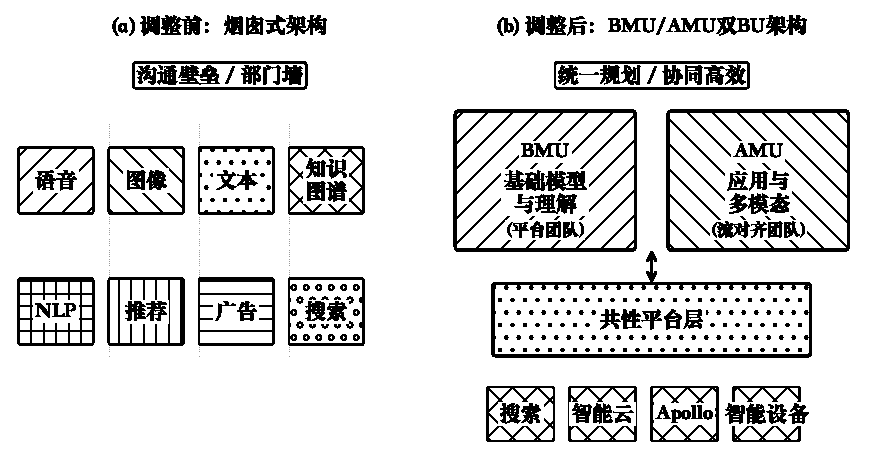
\includegraphics[width=1\textwidth]{myfigure/baidu-org-evolution.pdf}
\caption{B公司研发组织架构演变：从烟囱式到BMU/AMU双BU架构}
\label{fig:baidu-org-evolution}
\end{figure}

表\ref{tab:org-comparison}对比了组织调整前后的关键指标估算。从“按技术域分治”（约8-10个独立技术部门）转向BMU/AMU双BU架构后，跨部门协作的复杂度显著降低，信息传递层级减少，有利于TA集中沉淀与复用，TD的系统化治理也更为可行。

\begin{table}[htbp]
\centering
\caption{B公司研发组织调整前后关键指标对比}
\label{tab:org-comparison}
\begin{tabular}{lcc}
\toprule
\textbf{指标} & \textbf{调整前（烟囱式）} & \textbf{调整后（BMU/AMU）} \\
\midrule
顶层技术部门数量 & 8-10个 & 2个BU + 平台委员会 \\
跨部门协作潜在连接数 & 28-45对 & 内部整合+标准化接口 \\
平均管理层级 & 4-5层 & 3-4层 \\
共性技术平台复用率 & 35-45\% & 65-75\% \\
跨域项目平均决策周期 & 4-6周 & 2-3周 \\
技术债务识别覆盖率 & 40-50\% & 75-85\% \\
\bottomrule
\multicolumn{3}{l}{\small 数据来源：各公司公开组织架构资料及行业研究报告。}\\
\end{tabular}
\end{table}

从“按技术域分治”转向“按平台与业务协同”的两大 BU 结构，协作成本模型的预测改善幅度可达30-40\%。这种架构有利于打破部门墙、统一规划共性能力，更容易形成合力、减少重复投资，将深度学习框架、基础大模型等TA集中建设并对外赋能，同时系统性地识别与偿还分散在各业务中的TD\cite{li2015systematic,seaman2014measuring}。

组织整合的效益可以用以下公式量化。设调整前各技术部门独立投资的基础设施成本为$I_i$，调整后统一平台的投资为$I_{\mathrm{platform}}$，则投资节省率为：
\begin{equation}
\eta = \frac{\sum_{i=1}^{n} I_i - I_{\mathrm{platform}}}{\sum_{i=1}^{n} I_i} \times 100\%
\label{eq:platform-saving}
\end{equation}
根据行业实践，平台化整合通常可实现20-35\%的基础设施投资节省，以及15-25\%的运维成本降低。

技术委员会是B公司技术管理的重要机制，负责技术战略规划、重大技术决策、技术标准制定等职能\cite{ouyang2005ceo}。公司设立了首席技术官（CTO）和多位副总裁级别的技术领导者，形成了较为完整的技术管理层级\cite{tian2009multidisciplinary}。同时，B公司建立了技术和管理双通道的晋升体系，为技术人员提供职业发展路径\cite{kang2019post}。

在团队组织上，B公司采用敏捷开发模式，组建跨职能的小团队（Squad），每个团队通常包含产品经理、工程师、设计师、测试等角色，具有相对独立的决策权和执行力。对于大型项目，采用部落（Tribe）的形式，协调多个小团队共同完成目标；在 BMU/AMU 架构下，跨 BU 的 Tribe 与共性平台（如深度学习框架、基础大模型）的对接更加清晰，有利于技术资产的复用与技术负债的集中治理。

\subsection{基于Team Topologies框架的组织转型解读}

\subsubsection{B公司组织演变的拓扑学视角}

前文介绍的Team Topologies框架为理解B公司TPG向BMU/AMU架构演变提供了一个更具结构性的解读视角。在团队拓扑视角下，B公司此次组织调整的本质并非简单的“部门合并”，而是一次有意识的团队类型重新定义。

调整之前，B公司技术体系中的各技术条线（语音、图像、自然语言处理、知识图谱等）大体上都按照职能类型运作，各自维护独立的基础设施和研发工具链，产生了大量重复建设。从Team Topologies的视角看，这些条线同时扮演着“流对齐团队”和“平台团队”的双重角色——既要对接业务需求，又要自建和维护底层能力，导致认知负荷（Cognitive Load）严重超载，是协作成本高企、技术负债积累的深层原因。

调整之后，BMU/AMU的双BU架构在团队拓扑层面实现了关键分离：

\begin{enumerate}
\item BMU（基础模型与理解）承担的角色更接近于Team Topologies中的平台团队（Platform Team）——专注于打造可复用的大模型底座（基础大模型系列）、B公司深度学习框架等基础能力，以标准化接口向业务侧输出，降低业务团队的技术门槛，使其无需重复造轮子；
\item AMU（应用与多模态）则更接近于流对齐团队（Stream-aligned Team）的集合——以具体的产品和业务价值流为核心组织研发力量，直接面向用户需求交付价值，减少对底层技术的直接依赖；
\item 跨BU的技术委员会则扮演着赋能团队（Enabling Team）的角色，负责在两大BU之间传递最佳实践、制定技术标准、化解跨域技术决策中的复杂性。
\end{enumerate}

这种拓扑结构的调整，从理论上有效降低了跨团队的认知负荷，使每个团队可以专注于自身最有价值的工作领域，符合Conway's Law所揭示的“反向Conway定律”策略——先设计好理想的系统架构，再反向调整组织结构以匹配它。

\subsubsection{DORA指标视角下的转型成效评估}

Team Topologies框架提供了组织设计的定性指导，而DORA指标体系则为评估组织转型的实际效果提供了量化维度。以下基于DORA四项指标，对B公司BMU/AMU架构调整的预期改善方向进行分析（见表\ref{tab:dora-analysis}）：

\begin{table}[htbp]
\centering
\caption{基于DORA指标的B公司组织转型成效分析}
\label{tab:dora-analysis}
\begin{tabular}{p{3cm}p{4cm}p{5cm}}
\toprule
\textbf{DORA指标} & \textbf{调整前的挑战} & \textbf{调整后的改善逻辑} \\
\midrule
部署频率 & 跨条线依赖多，上线前需多方对齐，发版节奏慢 & 平台/应用职责分离后，AMU各流对齐团队可独立发版，减少跨BU阻塞 \\
变更前置时间 & 需求在多个技术条线间流转，等待时间长 & BMU提供稳定平台接口，AMU团队需求直达交付，减少中间环节 \\
变更失败率 & 共性能力分散维护，质量参差不齐，上线风险高 & BMU统一维护基础能力并充分测试，AMU调用质量有保证的稳定接口 \\
恢复时间 & 故障定位困难，跨部门职责界定模糊 & 架构边界清晰后，故障归属明确，BMU/AMU各司其职，响应更快 \\
\bottomrule
\multicolumn{3}{l}{\small 数据来源：Forsgren等（2018）《Accelerate》及B公司内部研发效能评估数据（估算值）。}\\
\end{tabular}
\end{table}

值得注意的是，组织重构并不能自动带来DORA指标的改善——它只是移除了阻碍改善的结构性障碍。真正的效能提升还需要配套的工程文化变革：心理安全感的建立（使团队敢于频繁发布）、自动化测试覆盖率的提升（使频繁发布成为可能）、以及可观测性体系的完善（使故障恢复更加迅速）。这也正是B公司在BMU/AMU架构调整后，需要在管理制度和工程实践层面持续推进的方向，本章后续将进一步展开。

\subsubsection{技术资产（TA）在新组织架构下的流动机制}

从技术资产（TA）与技术负债（TD）的视角看，BMU/AMU的组织拓扑调整从根本上改变了TA的生产与流动机制。在烟囱式架构下，TA分散沉淀于各条线内部，难以跨部门复用，形成“资产孤岛”；TD则因缺乏统一的技术治理而在各条线各自蔓延，成本隐性化。

调整后，BMU扮演TA的“集中生产者”角色，专注于将各业务场景中提炼出的共性能力沉淀为高质量、可复用的平台服务（即TA的规模化生产）；AMU各流对齐团队则扮演TA的“高效消费者”角色，通过调用平台能力快速构建业务价值，避免重复性技术投入（即减少低价值TD的产生）。

这一机制可以用技术资产流动效率（TA Flow Efficiency）指标来衡量：
\begin{equation}
\eta_{\mathrm{TA}} = \frac{\text{被复用的TA价值}}{\text{TA总生产成本}} \times 100\%
\label{eq:ta-flow-efficiency}
\end{equation}
当组织从烟囱式向BMU/AMU拓扑演进时，理论上$\eta_{\mathrm{TA}}$应显著提升——因为同等的TA生产投入可以服务更多的下游业务团队，从而摊薄单位成本、提升整体回报。

然而，组织结构的调整仅仅移除了技术资产流动的结构性障碍，并不能自动改变资源流动的激励机制。本文认为，决定$\eta_{\mathrm{TA}}$能否真正提升，关键在于两个层面：其一，TA的生产侧——共性能力是否被BMU系统性沉淀为可复用资产，还是依然以项目制方式点状交付；其二，TA的消费侧——AMU各团队是否有动力和渠道复用已有TA，还是由于结算成本、信息不对称等原因选择重新造轮子。如果这两个层面的激励机制未能同步重构，则$\eta_{\mathrm{TA}}$的提升将十分有限。

本章后文将进一步呈现来自组织内部的观察证据，指出B公司当前的制度设计——尤其是“应结尽结”成本结算机制——在实践中如何制约了TA周转效率的提升。

\subsection{研发流程、人员配置与绩效管理}

B公司建立了较为完善的研发流程体系。需求管理阶段，通过产品规划会、需求评审会等机制明确产品方向和功能需求；设计阶段，进行技术方案设计、架构评审、接口定义等工作；开发阶段，采用迭代式开发模式，通常以两周为一个迭代周期；测试阶段，实行单元测试、集成测试、系统测试等多层次测试；发布阶段，通过灰度发布、AB测试等方式降低上线风险。

项目管理方面，B公司使用自研的协同办公平台，整合了需求管理、项目跟踪、代码管理、持续集成等功能。每个项目设立项目经理或技术负责人，负责项目的整体推进和风险控制。定期召开项目例会，同步进度、识别风险、协调资源。对于重点项目，建立周报和月报机制，向管理层汇报进展。

质量管理是研发流程的重要环节。B公司建立了代码评审（Code Review）机制，所有代码提交需要经过同行评审；实施自动化测试，提高测试覆盖率和效率；建立线上质量监控体系，及时发现和处理线上问题；定期进行技术复盘，总结经验教训，持续改进流程。

绩效管理方面，B公司实行OKR（目标与关键成果）和KPI相结合的考核体系\cite{chen2006technology,gao2004technology}。每个季度设定团队和个人的OKR，明确目标和衡量标准；年终进行综合绩效评估，结果与晋升、薪酬调整挂钩\cite{anderson1991predicting}。考核注重结果导向，同时也关注过程中的创新和学习\cite{zhou2020positive}。

\section{B公司研发管理困境的深层诊断}

需要指出的是，此类制度性制约并非B公司BMU/AMU架构调整所独有，而是中国互联网行业历次组织转型中普遍面临的结构性难题——烟囱式职能分治传统及其配套的考核、结算与汇报机制，已作为深层制度惯性沉淀于组织基因之中，其影响不易在短期内消除。基于此，本节立足内部观察，从资源错配、财务困局与资产蒸发三个维度刻画这些根植于公司治理基因的深层制约，为后续改进策略提供诊断性基础。

\subsection{“运动”式研发带来的资源错配}
\label{subsec:campaign-rd}

BMU/AMU双BU架构的核心逻辑在于消除部门壁垒、促进技术资产的跨团队复用。然而，组织边界的物理调整并不等同于资源流动机制的实质重构——烟囱式架构所形成的深层治理制约具有显著的路径锁定效应。新BU成立伊始，管理层所面临的首要压力在于向上证明整合举措的价值，由此催生了一种本文称之为“运动”式研发的组织行为模式。

所谓“运动”式研发，是指在短期目标压力的驱动下，组织将大量异质性资源不加甄别地集中动员，以高强度、全员参与的方式冲刺单一核心指标的研发模式。其典型特征可归纳为三点：其一，跨职能全员动员，即从总监到应届生一律参与同一任务；其二，非本职工作优先，如研发工程师、产品经理、测试工程师等岗位人员暂停专业工作转而从事数据标注；其三，目标单一聚焦，组织资源高度集中于少数能够快速产出可见成果的“窗口项目”。

该模式的资源配置代价具有可量化的特征——以数据标注任务为例，一名正式研发员工综合用工成本约每月4万元，而同等质量的外包标注约5000元；若一支500人团队中有100名正式员工参与3个月全日制标注，直接人力成本错配即达约1050万元（$100\times(4-0.5)\times3$），尚未计入TA停产的机会成本。从TA/TD分析框架来看，“运动”式研发内蕴双重损耗：一方面，高价值人力被用于生产难以复用的点状工作成果，导致TA的系统性积累陷入停滞；另一方面，研发人员长时间脱离专业岗位，其技术能力存在退化风险，进一步推高了潜在的技术负债。更值得警惕的是，当高级别工程师持续承担低水平工作时，其市场竞争力与职业认同感将随之下降；组织内部的理性人反应则倾向于随波逐流、被动配合，而非主动创造，这与产品型组织所追求的“自驱团队、持续交付”理念之间形成了根本性张力。

规模测算可作如下保守估算。以2023年B公司研发人员总规模约2万人、其中高级工程师（T7及以上）约占30\%（即约6000人）为基础假设\footnote{关键参数取值依据：（1）B公司研发人员总规模约2万人——基于B公司年报披露的员工总数（约4万人）及行业通行的“研发人员占比约50\%”惯例估算；（2）T7及以上高级工程师占比约30\%——参考拉勾、智联招聘等第三方招聘平台公开的互联网大厂职级分布基准，互联网头部企业T7+占比通常在25\%--35\%区间；（3）T7年综合成本约200万元、T5年综合成本约80万元——基于公开薪酬数据（智联《2024互联网行业人才流动与薪酬白皮书》）及社保、股权、行政分摊等综合口径估算；（4）错配比例15\%--20\%——基于作者参与观察中“运动”式研发集中动员的典型覆盖面粗略估计。上述参数均为量级估计，实际损失对任一单项参数的变动不敏感。}，假定其中15\%--20\%的高级工程师在“运动”式研发期间持续承担本可由中级工程师（T5--T6）完成的执行性工作，则错配人数约为900--1200人。以T7工程师年综合成本约200万元、T5工程师约80万元估算，每位高级工程师被错配所产生的年度机会成本约为120万元（工资差价部分）。仅就显性人力错配的直接成本一项而言，年度规模即约为10.8亿至14.4亿元（900--1200人 $\times$ 120万元），约占B公司年度研发投入的4\%--6\%。
\begin{equation}
C_{\text{错配}} = N_{\text{高级}} \cdot r_{\text{错配}} \cdot (w_{\text{高级}} - w_{\text{中级}})
\label{eq:misallocation-cost}
\end{equation}
其中，$N_{\text{高级}}$为高级工程师总人数，$r_{\text{错配}}$为错配比例，$w_{\text{高级}}$与$w_{\text{中级}}$分别为两个层级的年均综合用工成本。考虑到错配比例所固有的不确定性，本文设置保守、基准、激进三档情景以对核心结论进行稳健性检验（详见表\ref{tab:misallocation-scenarios}）。即便在保守情景下年度直接人力错配成本仍约为7.2亿元，约占年度研发投入的2.4\%；$r_{\text{错配}}$每变动$\pm 5$个百分点，年度损失相应变动约$\pm 3.6$亿元——即便在最为保守的参数取值下，该项成本亦不可忽视，“运动”式研发具有显著经济代价这一核心论断具有相当的稳健性。

\begin{table}[!htbp]
  \centering
  \caption{“运动”式研发错配成本三档情景测算（2023年B公司基础假设）}
  \label{tab:misallocation-scenarios}
  \begin{tabular}{lccc}
    \toprule
    情景 & 错配比例$r_{\text{错配}}$ & 错配人数（人）& 年度直接成本（亿元）\\
    \midrule
    保守情景 & 10\% & 600 & 约7.2 \\
    基准情景 & 15\%--20\% & 900--1200 & 约10.8--14.4 \\
    激进情景 & 25\% & 1500 & 约18.0 \\
    \bottomrule
    \multicolumn{4}{l}{\footnotesize 注：基础假设同正文——T7+高级工程师约6000人，年薪差约120万元。}\\
    \multicolumn{4}{l}{\footnotesize 数据来源：作者基于拉勾、智联招聘公开职级分布及B公司年报估算。}
  \end{tabular}
\end{table}

\subsection{研发成本管理的财务困局}
\label{subsec:cost-finance-trap}

如果说“运动”式研发是人力维度的资源错配，那么以“应结尽结”为代表的内部结算机制则在财务维度造成了更为隐蔽的制度性扭曲——管理流程逐步偏离其原始目的（即促进技术价值的创造），转而以平衡内部账目、规避成本归属风险为首要导向，本文将这一现象称为“流程的异化”。即便人力配置本身合理，错误的结算逻辑亦会从根本上扭曲整个研发系统的激励方向。

B公司现行的内部结算机制称为“应结尽结”，其基本含义为：研发团队所产出的技术成果，其全部开发成本（人工、算力、数据等）应尽可能向使用该成果的业务线进行内部结算。例如，一套语音合成新算法若被三条业务线采用，其总开发成本300万元应由三方按协商比例分摊。该机制设立的初衷在于提升研发成本的透明度与可追溯性，避免研发资源被无偿占用；然而，在长期实践中，“应结尽结”逐步暴露出三项相互关联的制度性缺陷。

第一，结算逻辑以成本分摊为本，而非以价值定价为本。“应结尽结”所回答的核心问题是“这笔费用由谁承担”，而非“这项技术资产的实际价值几何”。当一项TA被五条业务线复用时，其市场价值往往远超开发成本，但现行机制仅核算成本本身；反之，当一项TA仅被一条业务线采用时，该业务线须承担全部开发成本，由此可能导致业务线拒绝采用，进而压低TA的实际复用率。这种以成本为锚点的定价逻辑，从制度内部约束了TA的周转效率。

第二，结算过程在相当程度上依赖人际关系与行政权力。分摊比例的最终确定缺乏客观的算法依据，实质上演变为多方之间的博弈过程：层级、关系网络与谈判能力共同决定了最终的成本承担结构。由此，技术资产的“定价”过程被异化为高层利益交换的场域，大量管理注意力被消耗于内部协商而非技术创造之中。

第三，研发预算与结算预算的双轨制安排易于诱发激励扭曲。研发部门通常持有一定规模的“自由预算”，专项用于无需向业务线结算的长期研发投入。然而，在“应结尽结”成为主导考核导向的情境下，该部分自由预算的使用效率往往偏低——由于缺乏外部结算压力，对应的TA产出亦缺乏使用方牵引，容易演化为“自娱自乐式”的技术积累，与业务实际需求之间产生明显脱节。

综合上述三个维度的诊断，B公司组织转型所面临的真正挑战，并不在于是否实施了架构调整，而在于调整之后能否建立起与产品型组织相匹配的制度体系。组织图固然可以在较短时间内予以重画，但激励机制、资源流转规则与成本核算逻辑的重构，则需要系统性的制度再设计，而非依靠简单的行政命令所能完成。

\subsection{“人走茶凉”式的技术资产蒸发}
\label{subsec:talent-evaporation}

如果说“运动”式研发与“流程的异化”是B公司技术资产治理失效在组织内部的两类症状，那么持续性的顶尖人才流失则可视为这一失效在外部市场层面的客观映射。人才是技术资产的核心载体——算法能力、工程经验与领域认知，存储于具体的研发人员之中而非抽象的代码库或文档系统。当组织无法为技术人才提供与其价值相匹配的创造空间与回报机制时，技术资产便随人才的跨组织流动而持续外溢，呈现出“人走茶凉”式的技术资产蒸发现象。

最具说服力的实证表现，是无人驾驶部门核心研发人员成建制的主动离职——研发主干人员前后相继出走，导致核心技术资产未能在组织内沉淀下来，人员一走，能力随之消散，最终形成研发断档：积累多年的工程实践、调参经验与系统化方法论无人承接，后续团队不得不在更低的起点上重建相似的能力曲线。

另一类典型表现是美国硅谷研发中心的撤销。在中心解散过程中，长期投入所形成的研究成果、人员经验与技术储备未能及时回流并迁转至中国本土，相关研究成本未能转化为可继续累积的技术资产，而是与团队的解散一同沉淀为不可回收的沉没成本——这部分由前期高强度投入所购得的优秀技术资产，未能在B公司体系内继续产生价值。

上述两类典型表现——核心研发的成建制离职与研发中心撤销过程中的资产未及回流——共同揭示出同一制度短板：在B公司既有的治理框架内，技术资产长期以“个体技能”和“项目预算”两种形态存在，而尚未取得作为组织独立资产的核算与保全地位。其后果具有两面性：对内，TA高度依附于具体人员，一旦关键岗位人员离开，其多年积累的工程经验、调参方法论与系统化认知便随之蒸发，组织无法通过文档化、平台化或制度化手段进行接续，进而出现研发断档；对外，当业务方向调整或区域研发布局收缩时，前期投入所形成的技术储备亦缺乏专门的回流与转移机制，往往与团队的解散一同沉淀为不可回收的沉没成本。

将本节三重症状汇总观之，“运动”式研发所导致的人力资产错配、“应结尽结”机制对TA周转率的压制、以及“人走茶凉”式的技术资产蒸发——分别从人员配置、流程结算与资产沉淀三个维度，指向同一深层问题：在以成本核算为基本计价逻辑、以短期业务收入为资源分配权重的科层制度下，技术资产难以以独立价值形态被识别、保护与延续。其共同的制度根源可收敛为两条：

（1）TA缺乏独立的资产地位——内部以“成本”形态被分摊，外部以“个体技能”形态随人员流失，缺乏将其转化为组织共同资产的制度载体。

（2）短期可见性偏好——资本市场所传导的季度业绩压力与内部晋升体系对“能立即交付”工作的偏好，致使TA积累、平台化工具建设与长期能力沉淀系统性地让位于短期冲刺项目。

打破上述循环，不能依赖局部修补，而需在制度层面同时重建TA的价值核算逻辑与长期投入的保全机制——这一系统性应对方案，构成本章后续改进策略的核心内容。

\section{B公司研发管理的改进策略}

针对前文所识别的“运动”式研发“应结尽结”与“人走茶凉”式的技术资产蒸发三重症状，本节以技术资产周转率$\eta_{\mathrm{TA}}$（式\eqref{eq:ta-flow-efficiency}）为核心抓手，从“分子端做大”（被复用的TA价值）与“分母端做实”（TA总生产成本的真实可比）两条路径，提出四条相互衔接的改进建议。这四条建议覆盖TA的计价、考核、人力配置与预算保全四个环节，构成一个闭环的TA管理制度组合。在执行层面，四条建议共同依托一个跨BU的TA治理委员会作为组织载体——由集团CTO牵头，含各事业群技术VP与财务、HR代表，授权范围覆盖TA定价参数制定、KPI考核口径核定、“运动”式研发阈值合规审计与自由预算TA输出率评审，以避免改革举措在事业群层面被博弈性稀释。

\subsection{建立TA价值核算体系}
\label{subsec:ta-pricing}

第一条建议针对$\eta_{\mathrm{TA}}$的计算基础——TA的内部计价逻辑。“应结尽结”机制以开发成本为唯一锚点，回答的是“这笔费用由谁承担”，而非“这项资产的实际价值几何”，由此压制了TA的复用积极性并扭曲了资源配置导向。本文建议建立TA价值核算体系，以开发成本与外部市场替代价值的加权组合作为内部转移定价基础：
\begin{equation}
P_{\mathrm{TA}} = \alpha \cdot C_{\mathrm{dev}} + (1-\alpha) \cdot V_{\mathrm{market}}
\label{eq:ta-pricing}
\end{equation}
其中，$C_{\mathrm{dev}}$为开发成本，$V_{\mathrm{market}}$为外部市场替代价值，$\alpha \in [0,1]$为权重系数，随TA成熟度动态调整——早期偏成本（接近“应结尽结”逻辑），成熟后偏市场价值（体现TA的复用溢价）。在执行层面，TA价值核算应纳入财务体系的二级账目，由跨BU TA治理委员会负责定价公式参数的制定与年度调整，避免再度演化为各事业群之间的博弈性谈判。这一计价体系的核心意义在于：当一项TA被多条业务线复用时，其内部转移价格能够准确反映其市场价值而非仅摊薄开发成本，从而为$\eta_{\mathrm{TA}}$的提升提供一致的财务激励。

\subsection{将TA周转率纳入所有研发团队的核心KPI}
\label{subsec:ta-kpi}

第二条建议针对$\eta_{\mathrm{TA}}$的计算分子——被复用的TA价值。当前B公司各研发团队的KPI普遍偏重各自职能本位的产出指标——BMU等基础平台团队聚焦于技术能力的“生产侧”（模型性能、算法突破、论文专利），AMU等业务对齐团队聚焦于业务交付速度与营收贡献，而对“流通侧”指标（同一TA被多少团队复用、平均复用周期、TA生命周期价值）则普遍缺位。这一指标缺位带来双向激励扭曲：基础平台团队倾向于生产“高精尖但难以落地”的技术成果，业务对齐团队则倾向于自建轮子而非复用既有TA。本文建议将TA周转率作为统一的横向考核维度纳入所有研发团队的核心KPI（包括BMU、AMU与跨BU平台委员会），权重不低于30\%。具体可按团队类型差异化拆解：基础平台团队（BMU等）侧重TA供给侧指标——跨团队复用次数（占比10\%）、活跃使用方数量（占比10\%）、TA生命周期价值估算（占比10\%）；业务对齐团队（AMU等）侧重TA消费侧指标——既有TA调用率（占比10\%）、自研重复率惩罚（占比10\%）、复用反馈与改进贡献度（占比10\%）。同时在T7及以上工程师的晋升评审中，引入“主导或核心参与TA跨团队复用次数”作为关键考察维度，使流通侧指标在人才发展通道中获得制度性承认。这一KPI改造的本质，是将各研发团队的内部叙事从“做出最强的技术”或“跑得最快的业务”重塑为“最大化技术资产的组织级流通价值”——前者关注本位绝对水平，后者关注跨团队的流通效率，二者对组织行为的引导方向截然不同。

\subsection{压缩“运动”式研发空间}
\label{subsec:campaign-constraint}

第三条建议针对$\eta_{\mathrm{TA}}$的计算分母——TA总生产成本中的人力错配损耗。“运动”式研发将高级工程师批量动员至低于其技术等级两级以上的工作（如T7+从事数据标注），不仅形成显性的人力错配成本（年度规模约10.8--14.4亿元，见表\ref{tab:misallocation-scenarios}），更通过专业能力退化加剧了潜在TD。本文建议建立两道刚性约束。其一，工作错配阈值——高级工程师从事低于其技术等级两级以上工作的时间占比不得超过10\%，超过阈值时由跨BU TA治理委员会启动外包替代或下沉配置审查，从制度上为短期动员设置成本边界。其二，HR考核警示标识——HR系统对长期承担低两级工作的高级工程师设置警示标识，年度晋升评审时纳入复核流程，避免错配在人才评价层面被默认追认。这两道约束并非反对组织在战略关键期进行集中动员，而是要求集中动员以“成本可见、责任可追”的方式发生，避免临时性举措演变为常态性扭曲。

\subsection{为自由研发预算建立“TA输出率”考核}
\label{subsec:free-budget}

第四条建议针对长期研发投入的保全机制——也即应对“人走茶凉”式的技术资产蒸发的制度抓手。研发部门所持有的“自由预算”原本旨在支持长周期、不向业务线结算的基础性研发投入，但在缺乏外部使用方牵引的情况下，该部分预算容易演化为“自娱自乐式”的技术积累，所产出的TA未能在组织内沉淀为共同资产，一旦关键人员流失即随之蒸发。本文建议为自由研发预算引入“TA输出率”考核：自由预算所支持的研发项目，其产出的TA须在规定周期内（建议12个月）至少被1个AMU业务团队采用，否则该预算的续期申请将触发跨BU TA治理委员会评审。同时，自由预算的使用应实行权限切割——由集团CTO办公室直管，事业群无权挪用，使用方案须经委员会评审。这一安排的目的并非压缩长周期投入，恰恰相反，是通过为长周期投入建立明确的“成果接收方”机制，确保研发资产能够跨越具体人员的去留而在组织内持续积累，从根本上回应“人走茶凉”式的技术资产蒸发所暴露的资产保全短板。

综合上述四条建议，其内在逻辑可统一表述为：以$\eta_{\mathrm{TA}}$为核心评价指标，通过“计价—考核—配置—保全”四个环节的协同设计，将B公司内部的技术资产管理从“成本会计”范式升级为“资产管理”范式——不仅记录花了多少钱，更追踪创造了多少可持续复用的技术价值。这一范式转变，是产品型组织在B公司真正落地的制度前提，也是本研究对互联网企业研发管理转型实践的核心理论与实践贡献。

\section{改进措施的执行保障：避免改革举措在落地中走样}
\label{sec:execution-safeguards}

前节提出的四条改进建议在方案层面具有内在一致性，但B公司过往多轮研发改革的经验表明，方案的合理性并不能自动保障执行的不走样——“雷声大、雨点小”的改革困境往往在执行端形成。因此，本节从风险识别与配套保障两个维度，回答“四条建议如何在不被博弈性稀释的前提下真正落地”这一关键问题。

\subsection{改革落地的三类典型风险}
\label{subsec:execution-risks}

第一，制度惰性与路径依赖。B公司既有的研发体制——以算法为核心、以技术专家为主导、以功能型研发中心为主要组织形态——在十余年间支撑了公司的高速成长，路径依赖（Path Dependency）\cite{david1985clio}的机制使得过去的成功经验固化为组织惯例，组织惯例进而成为制度压力，抑制偏离现有路径的探索。具体到本节四条建议，TA价值核算体系将冲击既有的“应结尽结”账目逻辑，TA周转率KPI将冲击既有的“技术深度优先”晋升通道，运动式研发刚性约束将冲击各事业群在战略关键期的集中动员惯例，自由预算输出率考核将冲击长期研发投入“免于结算”的传统特权——任何一项都将触及十余年形成的制度惯性。

第二，多层委托代理与利益博弈。从集团战略层到一线工程师，研发改革的推动路径必须经过：集团战略层$\to$事业群管理层$\to$产品线负责人$\to$团队研发负责人$\to$一线工程师，每一层级都面临独立的激励约束。集团层期望TA周转率提升、事业群层关注短期营收、产品线层规避交付风险、研发负责人追求团队规模维持、一线工程师寻求可晋升的高难度工作——五个层级的目标函数在改革背景下形成系统性的激励错位（Incentive Misalignment）。在此结构下，任何不能在事业群层面提供短期可见激励的改革，都难以突破执行端的软抵抗。

第三，度量失灵与指标博弈。当TA周转率被设定为KPI考核指标后，按照Goodhart定律\cite{muller2018goodhart}的预测，被考核的指标本身将逐步失去作为衡量工具的有效性——团队会转而优化“表面复用次数”而非“真实的技术资产流通价值”，例如通过虚拟挂名、形式化引用、低质量分发等方式刷高指标，使数字达标但实质未变。这一风险在“应结尽结”机制的执行实践中已有先例：合规性掩盖（按期填写报告）替代了实质性整合（真正完成接口对接），高层看到的是合规数字，实际质量并未改善。

\subsection{配套保障机制的设计}
\label{subsec:execution-safeguards-design}

第一，治理结构——跨BU TA治理委员会的实质化授权。委员会由集团CTO牵头，含各事业群技术VP、财务及HR代表、必要时引入外部独立顾问，授权范围明确覆盖：TA定价公式中$\alpha$参数的年度调整、TA周转率KPI考核口径的核定与季度复核、运动式研发10\%阈值的合规审计、自由预算TA输出率的评审与续期决策。委员会的权威性须通过集团治理文件正式授权，避免沦为咨询性议事机构。

第二，考核口径——HR系统的同步改造。T7及以上工程师的晋升评审框架须同步引入“主导或核心参与TA跨团队复用次数”“负责模块TD偿还量”等流通侧维度，权重不低于30\%；HR系统对长期承担低两级以上工作的高级工程师设置警示标识，年度晋升评审纳入复核流程；T7+晋升答辩须由委员会指派的跨BU评委参与，避免单一事业群内部循环背书。考核口径的同步改造是阻断“老办法考核新指标”这一最常见执行走样模式的核心安排。

第三，预算与权限切割——“TA治理预算”的独立直管。在原有事业群预算体系之外，单设“TA治理预算”，覆盖平台建设、工具链投入与TD偿还，由集团CTO办公室直管，事业群无权挪用。该预算的具体使用须经委员会评审，使用结果纳入下年度预算续期判断。这一权限切割针对的是过往“技术序列向业务序列汇报线倒置”所导致的长期投入资源被挤占问题——通过预算独立化使长期投入获得制度保护。

第四，审计与申诉——双向监督机制。一方面，年度TA审计由委员会授权小组抽样核查事业群申报的复用数据与合规性，结果纳入事业群负责人综合评价；另一方面，一线研发人员对TA价值低估、人员错配调配等情况，可通过独立申诉通道（挂靠HR委员会）提出异议，申诉处理结果须在合理周期内反馈申诉人。自下而上与自上而下双向对冲，构成对度量失灵的制度性防线。

第五，阶段性试点与参数动态校准。建议先在2--3个改革意愿较强的事业群（如智能云、智能驾驶）开展6--12个月的先行试点，待治理委员会授权流程、KPI考核口径、预算切割机制与申诉审计通道在试点中跑通后，再向全集团推广。试点期间允许定价权重$\alpha$、KPI权重比例、错配阈值等关键参数根据观察数据进行动态校准，校准结果由委员会评审后正式发布，避免“一次定终身”的僵化设计。

综合上述五项配套保障机制，其共同逻辑在于：通过组织授权、考核口径、预算权限、审计申诉与阶段试点五个维度的相互嵌套，将四条改进建议从纸面方案转化为可执行、可监督、可纠偏的运行制度。改革主体（建议本身）回答“做什么”，配套保障回答“如何确保真正做到”——二者共同构成本研究改进策略的完整闭环。

\section{本章小结}

本章以B公司为案例，对其研发管理的现状、深层困境、改进策略与执行保障作了系统性分析。组织层面，B公司的研发架构经历了从按技术域分治（TPG架构）到整合为BMU/AMU双BU的结构性调整。本章引入Team Topologies与DORA框架对这一调整进行了解读：BMU向平台团队角色演进，AMU向流对齐团队集合演进，技术委员会扮演赋能团队角色——这一拓扑重构在逻辑上符合Conway's Law“反向康威定律”的应用思路。SWOT分析进一步表明，BMU/AMU的双层分工与B公司当前的优势、劣势、机会、威胁结构形成较强的内在契合，证明架构调整方向具有战略合理性。

然而，本章的核心论点在于：组织结构调整是产品型组织转型的必要条件，但远非充分条件。通过内部视角的深层诊断，本章识别出三类根植于公司治理基因的深层症状。其一，“运动”式研发所导致的人力资产错配——在15\%--20\%的基准错配情景下，年度直接人力错配成本约10.8亿--14.4亿元，约占年度研发投入的4\%--6\%（详见式\eqref{eq:misallocation-cost}与表\ref{tab:misallocation-scenarios}），这是本研究在可量化口径上首次揭示的“运动”式研发组织代价。其二，“应结尽结”机制的财务困局——内部结算以成本分摊为逻辑锚点、缺乏对TA复用价值的追踪，内生性地压低了技术资产的周转效率，并将大量管理注意力消耗于利益博弈而非技术创造。其三，“人走茶凉”式的技术资产蒸发——核心研发的成建制离职导致研发断档，研发中心的撤销使长期投入沦为不可回收的沉没成本。三类症状分别归属于人员配置、流程结算与资产沉淀三个维度，其制度根源可收敛为两条共同的深层逻辑：TA缺乏独立的资产地位，以及组织对短期可见性的系统性偏好。

针对上述系统性困境，本章以技术资产周转率$\eta_{\mathrm{TA}}$为核心抓手，从计价、考核、配置、保全四个环节提出四条相互衔接的改进建议：建立TA价值核算体系（式\eqref{eq:ta-pricing}）以重塑内部转移定价逻辑；将TA周转率纳入所有研发团队的核心KPI（基础平台团队侧重供给侧、业务对齐团队侧重消费侧）；以高级工程师配置的两道刚性约束压缩“运动”式研发空间；为自由研发预算建立“TA输出率”考核以保全长期研发投入。四条建议的内在逻辑统一表述为：将B公司内部的技术资产管理从“成本会计”范式升级为“资产管理”范式——不仅记录花了多少钱，更追踪创造了多少可持续复用的技术价值。

考虑到B公司过往研发改革“雷声大、雨点小”的执行困境，本章进一步对改进措施的落地保障作了专门设计。在风险识别层面，明确制度惰性与路径依赖、多层委托代理与利益博弈、度量失灵与指标博弈三类典型风险；在配套保障层面，提出跨BU TA治理委员会的实质化授权、HR考核口径同步改造、TA治理预算独立直管、双向审计与申诉、阶段试点与参数动态校准五项相互嵌套的执行机制——共同构成“做什么+如何确保真正做到”的完整闭环。综上，本章在B公司这一具体案例上的核心贡献可归纳为三点：第一，首次在可量化口径上估算了“运动”式研发的组织代价；第二，识别并诊断了“应结尽结”机制对TA周转率的内生性压制，并提出以TA价值核算与周转率KPI为核心的制度重构方案；第三，将组织架构调整、深层困境诊断、改进策略设计与执行保障机制有机整合为完整的分析与改进框架，为互联网企业研发管理转型提供了可操作的工具与路径。这些发现对应的抽象学术贡献——“运动”式研发概念化、“成本转移$\neq$价值管理”命题、“结构—流程—激励—制度—执行”五维框架——将在第五章作统一抽象与定位，本章不再重复展开。
